%--------------------------------------------------
\section{MARCO TEÓRICO}
La pobreza multidimensional reconoce que las privaciones que enfrentan los hogares trascienden el ingreso e incluyen dimensiones como salud, educación, vivienda, servicios básicos y empleo. En Colombia, su medición oficial se realiza mediante el Índice de Pobreza Multidimensional (IPM), lo que permite identificar privaciones específicas y orientar intervenciones focalizadas. Sin embargo, la disponibilidad territorial del IPM es limitada: salvo la estimación derivada del Censo 2018, no existen mediciones periódicas para los 1.122 municipios del país. Esta brecha de información dificulta el diagnóstico local y la formulación de políticas basadas en evidencia, especialmente en zonas con baja representatividad estadística. Este vacío metodológico motiva el uso de técnicas capaces de producir estimaciones confiables a nivel municipal mediante fuentes auxiliares, como la Estimación para Áreas Pequeñas (SAE).

Los modelos SAE ofrecen una base estadística sólida para generar estimaciones precisas en dominios con escasa muestra, mediante la integración de información proveniente de censos, registros
administrativos y encuestas \cite{CEPAL_PovertyMapping_2022}. Existen dos grandes enfoques: los modelos de área, como el modelo
Fay–Herriot, que utilizan estimaciones directas agregadas y covariables auxiliares; y los modelos de unidad, que emplean microdatos para capturar variabilidad individual. La selección depende de la calidad y granularidad de las fuentes disponibles, pero ambos enfoques permiten mejorar la precisión, reducir la varianza y generar estimaciones territorialmente consistentes, lo cual es fundamental en contextos municipales.

No obstante, cuando los indicadores presentan patrones territoriales no explicados completamente por las covariables, resulta necesarioenfoques espaciales que modelen explícitamente la dependencia geográfica. Los modelos espaciales integran estructuras de vecindad o efectos aleatorios espaciales, lo que permite “suavizar” las estimaciones entre municipios contiguos y reducir variabilidad no explicada. La literatura demuestra que estos modelos mejoran la coherencia territorial, especialmente en dominios pequeños y heterogéneos como los municipios colombianos \cite{PratesiSalvati_2019}.

Las herramientas de ciencia de datos complementan este proceso al facilitar la selección de variables auxiliares, el análisis de relaciones no lineales y la integración de datos heterogéneos, incluyendo fuentes satelitales como VIIRS. Asimismo, la visualización interactiva (a través de dashboards y mapas
temáticos) constituye un elemento clave para la interpretación y difusión de resultados, permitiendo a instituciones y tomadores de decisión explorar patrones territoriales de manera más accesible.

La aplicación de modelos SAE y de sus extensiones espaciales depende directamente de la disponibilidad de covariables confiables y de cobertura completa. En este proyecto se emplearán fuentes oficiales como el Censo Nacional de Población y Vivienda 2018, la GEIH y la ECV del DANE, registros administrativos sectoriales y datos geoespaciales abiertos. A partir de estas fuentes se derivarán variables relacionadas con condiciones de vivienda, servicios públicos, educación, entorno e infraestructura, esenciales para mejorar la capacidad predictiva del modelo y compensar la baja representatividad muestral en muchos
municipios.

En conjunto, los enfoques revisados —modelos SAE, modelos espaciales, herramientas de ciencia de datos y visualización— constituyen el fundamento conceptual que sustenta este proyecto. Su
integración permite generar estimaciones municipales del IPM más precisas y territorialmente coherentes, aportando una base metodológica adecuada para el análisis territorial en contextos con
limitaciones de información estadística.

%--------------------------------------------------
%\section{Fundamento teórico de ciencia de datos}
%\label{sec:Fundamento-teorico}

%    %--------------------------------------------------
%    \subsection{Modelo 1}

 %   \begin{equation}
 %   \begin{aligned}
 %       \operatorname{Bin}(y_i \mid n_i, \theta_i)
 %       &\propto \theta_i^{y_i} (1 - \theta_i)^{n_i - y_i} \\
 %       &\propto \exp(\eta_{i 1})^{y_i} / (1 + \exp(\eta_{i 1}))^{n_i} \\
 %       &\propto (e^\psi)^a / (1 + e^\psi)^b
 %   \end{aligned}
 %   \label{eq:binomial-likelihood}
 %   \end{equation}
    
    
 %   %--------------------------------------------------
 %   \subsection{Modelo 2}
    
    
    
    % \begin{figure}[!htbp]
    %     \centering
    %     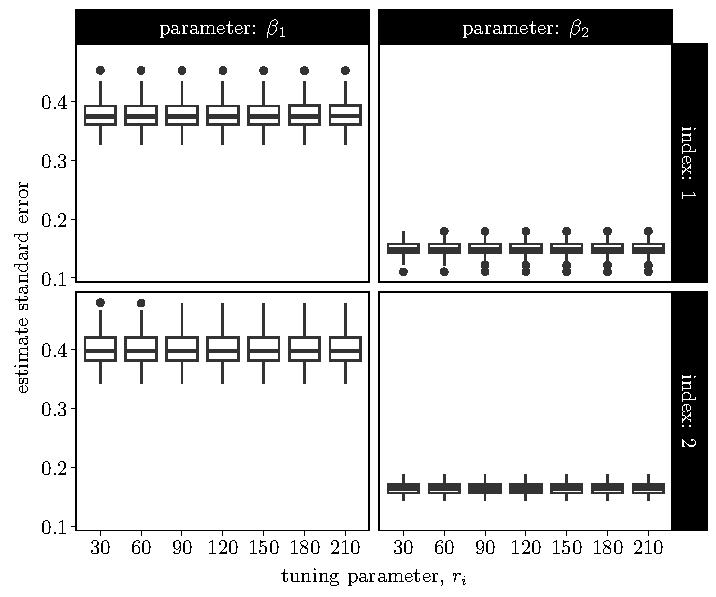
\includegraphics[width=0.75\textwidth]{fig/fig_new_experiment_01.pdf}
    %     \caption{Estimate standard errors as a function of the tuning parameter $r_i$. The standard errors are relatively stable across values of $r_i$.}
    %     \label{fig:fig_new_exp_01}
    % \end{figure}